\section{Method}

\subsection{System Architecture}

Both extensions are built on the DeepMTL2R framework, whose baseline pipeline consists of an input layer, a transformer encoder, and a task-specific output layer, as illustrated in Figure~\ref{fig:baselinepipeline}. Input features are first projected through a shared \texttt{FCModel}, then encoded using self-attention \cite{vaswani2017attention} across the query slate, and finally passed to task-specific linear heads that each generate a scalar relevance score.
\begin{figure}[!htbp]
  \centering
  \includegraphics[width=\columnwidth]{images/DeepMTL2R.png}
  \caption{DeepMTL2R baseline pipeline.}
  \label{fig:baselinepipeline}
\end{figure}

\subsubsection{Dynamic Feature Gating}

Dynamic Feature Gating introduces a trainable gating mechanism directly before \texttt{FCModel}, acting as a soft feature-selection mask, as shown in Figure~\ref{fig:featuregating}.
\begin{figure}[!htbp]
  \centering
  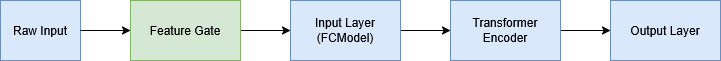
\includegraphics[width=\columnwidth]{images/FeatureGating.png}
  \caption{DeepMTL2R architecture modified with Dynamic
  Feature Gating.}
  \label{fig:featuregating}
\end{figure}

Let $\mathbf{x} \in \mathbb{R}^d$ denote the raw input feature vector with dimensionality $d = 133$. A linear transformation followed by a sigmoid activation is applied to generate the gating mask, given by
\begin{equation}
  \mathbf{g} = \sigma(\mathbf{W}_g \mathbf{x} +
  \mathbf{b}_g), \quad \mathbf{g} \in [0, 1]^d\text{,}
\end{equation}
after which the gated representation is obtained through the element-wise Hadamard product
\begin{equation}
  \mathbf{\tilde{x}} = \mathbf{g} \odot \mathbf{x}\text{.}
\end{equation}

\subsubsection{Matryoshka Feature Projection}

Matryoshka Feature Projection integrates Matryoshka
Representation Learning (MRL) \cite{kusupati2022matryoshka}
into the output projection layer
(Figure~\ref{fig:matryoshka}), widening the encoder
hidden size to $D = 256$ and enforcing coarse-to-fine
encoding via nested prefix slices.

\begin{figure}[!htbp]
  \centering
  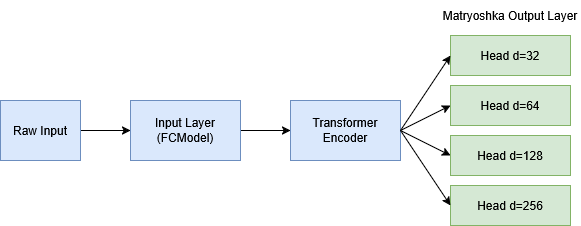
\includegraphics[width=\columnwidth]{images/Matryoshka.png}
  \caption{DeepMTL2R architecture modified with
  Matryoshka Feature Projection.}
  \label{fig:matryoshka}
\end{figure}

For nesting dimensions $\mathcal{M} = \{32, 64, 128, 256\}$, each slice $\mathbf{h}^{(m)} = \mathbf{h}_{1:m}$ is connected to a task-specific linear prediction head such that
\begin{equation}
  \hat{y}_t^{(m)} = \mathbf{w}_{t}^{(m)\top}
  \mathbf{h}^{(m)} + b_t^{(m)} \text{,}
\end{equation}
where $t \in \mathcal{T} = \{0,1,2,3\}$. The overall training objective is then obtained by aggregating the losses across all nesting dimensions and tasks, yielding
\begin{equation}
  \mathcal{L}_{\text{total}} = \sum_{m \in \mathcal{M}}
  \sum_{t \in \mathcal{T}} w_t \mathcal{L}_t\!\left(
  \hat{\mathbf{y}}_t^{(m)}, \mathbf{y}_t\right)\text{.}
\end{equation}
At inference time, only the full $D = 256$ slice is used by default, although lower-dimensional sub-vectors can still be extracted for latency-critical retrieval scenarios.

\subsection{Training Hyperparameters}

All architectures share the hyperparameters listed in
Table~\ref{tab:hyperparams}. Training uses the LambdaLoss framework \cite{wang2018lambdaloss} with \texttt{ndcgLoss2PP\_scheme} ($\mu=10$, $\sigma=1.0$), the Adam optimizer (lr $= 0.001$), and a batch size of 32 query slates over 50 epochs.

\begin{table}[h]
  \centering
  \caption{\label{tab:hyperparams}
    Training hyperparameters shared across all
    architectures.
  }
  \resizebox{\columnwidth}{!}{%
  \begin{tabular}{lll}
    \toprule
    \textbf{Hyperparameter} & \textbf{Value} &
    \textbf{Description} \\
    \midrule
    Epochs        & 50       & Max training epochs \\
    Batch size    & 32       & Query slates per batch \\
    Optimizer     & Adam     & Adapts learning rates
                               per parameter \\
    Learning rate & 0.001    & Initial LR \\
    LR scheduler  & StepLR  & \texttt{step\_size=50},
                               \texttt{gamma=0.1} \\
    Loss function & LambdaLoss &
                    \texttt{ndcgLoss2PP\_scheme},
                    $\mu=10$ \\
    \bottomrule
  \end{tabular}%
  }
\end{table}